\documentclass[11pt,a4paper]{book}   % or report/article
\usepackage[utf8]{inputenc}
\usepackage[T1]{fontenc}
\usepackage[english]{babel}
\usepackage{amsmath,amssymb,amsthm,mathtools}
\usepackage{graphicx}
\usepackage{algorithm,algpseudocode}
\usepackage{caption}
\usepackage[most]{tcolorbox}
\usepackage{float}

\usepackage{tikz}
\usetikzlibrary{arrows.meta, positioning}
\usepackage{stmaryrd}   % for the \mapsfrom arrow
\usepackage{subcaption}

\newtcolorbox[auto counter, number within=chapter]{esempio}[1]{
  enhanced, breakable,
  colback=blue!4,
  colframe=blue!55!black,
  boxrule=0pt, frame hidden,
  borderline west={3pt}{0pt}{blue!55!black},
  sharp corners,
  coltitle=blue!55!black,
  colbacktitle=blue!10,
  fonttitle=\bfseries,
  title={Example~\thetcbcounter: #1},
  before skip=1em, after skip=1em
}

\newtcolorbox[auto counter, number within=chapter]{algobox}[1]{
  enhanced, breakable,
  colback=gray!5,
  colframe=gray!60!black,
  boxrule=0pt, frame hidden,
  borderline west={3pt}{0pt}{gray!60!black},
  sharp corners,
  coltitle=gray!20!black,
  colbacktitle=gray!20,
  fonttitle=\bfseries,
  title={Algorithm~\thetcbcounter: #1},
  before skip=1em, after skip=1em
}

\newtcolorbox[auto counter, number within=chapter]{defbox}[1]{
  enhanced, breakable,
  colback=green!4!white,
  colframe=green!45!black,
  boxrule=0pt, frame hidden,
  borderline west={3pt}{0pt}{green!45!black},
  sharp corners,
  coltitle=green!35!black,
  colbacktitle=green!12!white,
  fonttitle=\bfseries,
  title={Definition~\thetcbcounter: #1},
  before skip=1em, after skip=1em
}
\usepackage{dsfont}

\definecolor{arrowblue}{RGB}{68,114,196}

% lines, labels and limit point shared by both diagrams
\newcommand{\gpibase}{%
  \coordinate (P) at (6,0);
  \draw[thick] (0,2.4) -- (P);
  \draw[thick] (0.7,-1.22) -- (P);
  \node[above, rotate=-21.8, font=\footnotesize] at (2.95,1.3) {$\mathrm{v} = \mathrm{v}_\pi$};
  \node[below, rotate=13, font=\footnotesize] at (2.9,-0.7) {$\pi = \text{greedy}(\mathrm{v})$};
  \node[right, font=\footnotesize] at (6.05,0) {$\mathrm{v}_*, \pi_*$};
  \node[below, font=\footnotesize] at (0,0.55) {$\mathrm{v}, \pi$};
}

\usepackage{booktabs}
\usepackage{tabularx}
\usepackage{longtable}
\usepackage{colortbl}

\setcounter{secnumdepth}{3}   % number down to subsubsection
\setcounter{tocdepth}{3}      % and show it in the table of contents

\newtheorem{theorem}{Theorem}[chapter]
\newtheorem{definition}[theorem]{Definition}
\newtheorem{lemma}[theorem]{Lemma}

% Handy RL macros
\newcommand{\E}{\mathbb{E}}
\newcommand{\R}{\mathbb{R}}
\DeclareMathOperator*{\argmax}{arg\,max}
\newcommand{\pol}{\pi}
\newcommand{\Q}{Q^{\pi}}

% hyperref and cleveref must be loaded last
\usepackage{hyperref}
\usepackage{cleveref}


\title{Reinforcement Learning Notes}
\author{Maurizio Camposeo \and Daniele Di Spirito}
\date{\today}

\begin{document}
\maketitle
\tableofcontents

% !TEX root = ../main.tex
\chapter{Introduction}
\section{Machine Learning}
Machine Learning based technologies solve specific tasks very well, while AI chatbots have quite broad and general capabilities.
However classic machine learning predictions may not be sufficient for decision-making. 
Machine learning requires a 'supervisor' that provides meaningful data of the phenomenon we want to characterize. Typically we need $(x, y)$ and we look for a relationship $F$.
In many scenarios this is not feasible. 

RL aims to solve cases where data must be collected 'in the wild' (agent interacts with the world and learns how to maximize some objectives).

\section{Limits of Supervised Learning}
There are some limits for supervised learning techniques like RL:
\begin{itemize}
    \item Data are not aviable without interacting with the world;
    \item Collected data may not be explicitly associated to an action;
    \item Time matters: we don't always have i.i.d. data;
    \item In many settings, supervised learning do not envision long-term scenarios.
\end{itemize}

\section{RL Formalism}
\begin{itemize}
    \item An \textbf{agent}: entity aiming at solving the task;
    \item A set of \textbf{states ($\textit{S}$)} in which the agent can be;
    \item A set of \textbf{actions $(\textit{A})$} that can be taken by the agent;
    \item An \textbf{environment} with which the agents interacts, and that changes after the agent takes an action (also provides back a \textbf{reward $(\textit{R})$});
    \item The agent can be more interested in long-term rewards more than short-term.
\end{itemize}

\begin{figure}[htbp]
    \centering
    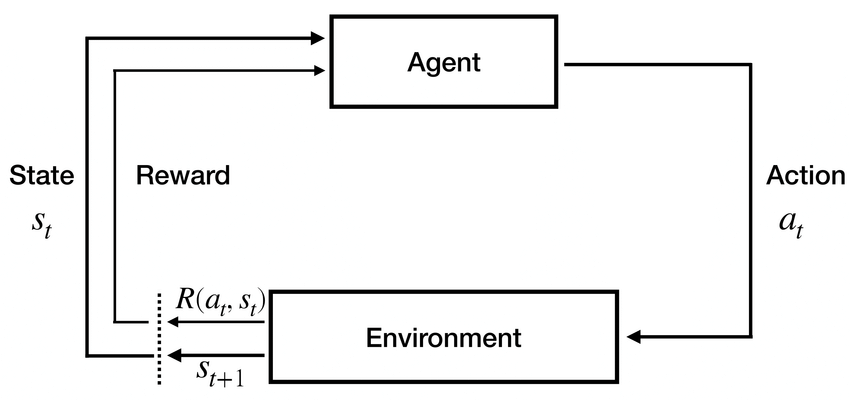
\includegraphics[width=0.7\textwidth]{./figures/chapter1/Reinforcement-Learning-framework-adapted-from-Sutton-and-Barto-2018-1915045654.png} 
    \caption{Markov Decision Process scheme.}
    \label{fig:MDP}
\end{figure}

\section{RL Problem}
The agent could initially know very little about the environment and about which reward and next states a give action from a given state could lead to. In other terms the dynamics of the environment is not known in advance, they must be learned by interaction with the environment.
The goal of the agent is to maximize long term rewards. 
% !TEX root = ../main.tex
\chapter{RL Elements and Multi-Armed Bandits}

\section{The RL Elements}
\subsection{Reward}
A reward $R_t$ is a scalar feedback that indicates how well the agent is doing at step $t$.
Step $t$ indicates a discrete time-step (a continuous-time treatment is possible but not considered in this course).
We consider a time-step in:
\begin{enumerate}
    \item \textbf{Episodic tasks:} last for a finite amount of time;
    \item \textbf{Continuing tasks:} never end and continue indefinitely.
\end{enumerate}
The agent's job is to maximize the \textit{cumulative reward}:
\begin{enumerate}
    \item In episodic tasks, cumulative reward over an episode;
    \item In continuing tasks, cumulative reward over a defined horizon (that can be rolling).
\end{enumerate}
RL is based on the \textit{reward hypothesis}:
\begin{center}
  \itshape ``All goals can be described by the maximization of expected cumulative reward.''
\end{center}
Actions may have long-term consequences and rewards may be delayed: immediate rewards can be sacrificed to gain more long term rewards.

\subsection{The Agent and the Environment}
At each step $t$ the agent is in the state $S_t$ and takes an action $A_t$ that is a feasible action from that state. The environment, based on the state-action pair $(S_t, A_t)$, returns a reward $R_{t+1}$ and moves the agent in the state $S_{t+1}$.

\subsection{Observation and History}
Moreover, at each step the agent sees an \textit{observation} $O_{t+1}$:
\begin{itemize}
    \item In \textit{fully observable environments} $S_{t+1}=O_{t+1}$;
    \item In \textit{partially observable environments} the state is not available and must be inferred from the history:
    \[H_t=O_1,R_1,A_1,...,A_{t-1},O_t,R_t\]\[S_t=f(H_t)\] 
\end{itemize}
If we can't have a reliable state we must define different strategies (taking whole history as state or estimate the state with a supervised learning approximation).

\subsection{Components of an Agent}
An agent may have the following components:
\begin{itemize}
    \item (always) a \textit{policy}, the function that describes the behavior of the agent and maps states to actions. The RL goal is to find the optimal policy. Policy can be:
        \begin{itemize}
            \item \textit{Deterministic policy}, $a=\pi(s)$
            \item \textit{Stochastic policy}, $\pi(a|s)=P[A_t=a|S_t=s]$
        \end{itemize}
    \item (possibly) a \textit{value function}, a quantitative description of how good each state is;
    \item (possibly) a \textit{q-value function}, a quantitative description of how good a (state,action) pair is;
    \item (possibly) a \textit{model}, the agent's representation of the environment.
\end{itemize}

\section{Multi-armed Bandits}
In this case we consider simple settings where there is only one state ($S_t=S_{t+1}$) and the agent has to choose among $k$ actions (arms of a bandit). The agent's goal is to maximize the expected reward over time. The agent must balance exploration (trying new actions) and exploitation (choosing the best-known action).

In the example of slot machines (`one-armed bandits'), each machine is associated with a different probability distribution of rewards. At each episode the agent can pull only one lever. The aim is to understand the best strategy to maximize cumulative rewards over different episodes. 

\subsection{Action Values}
Each action provides a stochastic reward, and the q-value of an action is the following (we are considering that the state never changes):
\[q_*(a)\doteq\mathbb{E}[R_t\mid A_t=a]\]
In this case $t$ indicates the episode number, while in typical RL settings it indicates the time-step within an episode.

The q-value for an action is not known and must be estimated, a simple way is by the \textit{Sample-Average} method:
\[Q_t(a)\doteq\frac{\text{sum of rewards when }a\text{ is taken prior to }t}{\text{number of times }a\text{ is taken prior to }t}=\frac{\sum_{i=1}^{t-1}R_i\cdot\mathds{1}_{A_i=a}}{\sum_{i=1}^{t-1}\mathds{1}_{A_i=a}}\]
where $\mathds{1}_{\text{predicate}}$ equals 1 if the predicate is true and 0 otherwise. Every time I collect a new data point I can recompute this estimate.

\subsection{Incremental Implementation of Action Value Estimate}
If we consider a single action $a$ and $R_i$ the reward received after the $i$-th selection of $a$, after $n-1$ selections of action $a$ we can estimate its action value as:
\[Q_n\doteq\frac{R_1+R_2+\cdots{}+R_{n-1}}{n-1}\]
This approach is not efficient because memory and computation will grow over time.
\begin{equation}
\begin{split}
  Q_{n+1}&=\frac{1}{n}\sum_{i=1}^{n}R_i \\
  &=\frac{1}{n}\left(R_n+\sum_{i=1}^{n-1}R_i\right) \\
  &=\frac{1}{n}\left(R_n+(n-1)Q_n\right) \\
  &=\frac{1}{n}\left(R_n+nQ_n-Q_n\right) \\
  &=Q_n+\frac{1}{n}\left(R_n-Q_n\right)
\end{split}
\end{equation}
This implementation requires only $Q_n$ and $n$ to compute $Q_{n+1}$, we don't need all the past values of the rewards.
The more rewards I see, the less relevant the `innovation' is (not ideal for non-stationary problems).
For this reason we move to a step-size that does not change over time (typically $\alpha\in(0,1]$).
\[\textit{NewEstimate}\leftarrow\textit{OldEstimate}+\textit{StepSize}\left[\textit{Target}-\textit{OldEstimate}\right]\]
In this way I also don't need to keep track of the number of times an action has been selected, but I need to choose a step-size $\alpha$. The result is an \textit{exponential recency-weighted average}, which gradually forgets old rewards. This is convenient for \textit{non-stationary} problems where the reward distribution of the actions changes over time.
\begin{equation}
\begin{split}
  Q_{n+1}&=Q_n+\alpha\left(R_n-Q_n\right) \\
  &=\alpha R_n+(1-\alpha)Q_n \\
  &=\alpha R_n+(1-\alpha)\left[\alpha R_{n-1}+(1-\alpha)Q_{n-1}\right] \\
  &=\alpha R_n+\alpha(1-\alpha)R_{n-1}+(1-\alpha)^2Q_{n-1} \\
  &=\alpha R_n+\alpha(1-\alpha)R_{n-1}+\alpha(1-\alpha)^2R_{n-2}+ \\ &\cdots{}+\alpha(1-\alpha)^{n-1}R_1+(1-\alpha)^nQ_1 \\
  &=(1-\alpha)^nQ_1+\sum_{i=1}^{n}\alpha(1-\alpha)^{n-i}R_i
\end{split}
\end{equation}
\subsection{Greedy Policy}
With a greedy policy the selected action will be:
\[A_t\doteq\argmax_{a}Q_t(a)\]
This policy is the simplest one, but it does not explore: we may get stuck with a suboptimal action.

\subsection{Exploration vs Exploitation}
\textit{Exploration} allows us to improve knowledge for long-term benefit, while \textit{Exploitation} exploits knowledge for short-term benefit.
We cannot explore and exploit at the same time, so implementing a trade-off is necessary to avoid suboptimal solutions. There are different approaches to cope with the trade-off:
\begin{itemize}
    \item $\varepsilon$-greedy;
    \item greedy with optimistic initialization;
    \item Upper Confidence Bound (UCB);
    \item Gradient Bandit.
\end{itemize}

\subsubsection{\texorpdfstring{$\boldsymbol{\varepsilon}$}{epsilon}-Greedy Policy}
This is a stochastic policy, defined as follows:
\begin{equation}
  A_t\overset{\text{def}}{=}
  \begin{cases}
    \text{greedy action with probability }1-\varepsilon\\
    \text{a random action among all }k\text{ with probability } \varepsilon
  \end{cases}
\end{equation}
with $\varepsilon\in(0,1)$ (typically a small number). In the random case the action is chosen uniformly among all $k$, including the greedy one.

\begin{esempio}{The 10-armed testbed}
Consider \textbf{2000 randomly generated} 10-armed bandit problems.

\medskip
\noindent\textbf{Generating a problem.}
For each problem, the true action values are drawn as
$q_*(a) \sim \mathcal{N}(0,1)$ for $a = 1,\dots,10$.
When the agent selects action $a$, it receives
$R \sim \mathcal{N}(q_*(a),\,1)$.

\medskip
\noindent\textbf{What the agent does.}
In each problem the agent starts with all estimates set to zero and plays
$1000$ steps, updating $Q_t(a)$ along the way. There is no memory
between one problem and the next (independent problems).

\medskip
\noindent\textbf{Evaluation.}
At each step $t$, performance is averaged over the 2000 problems:
\[
  \bar{R}_t = \frac{1}{2000}\sum_{k=1}^{2000} R_t^{(k)}
  \qquad
  \%\text{ optimal}_t = \frac{1}{2000}\sum_{k=1}^{2000}
  \mathds{1}_{A_t^{(k)} = \arg\max_a q_*^{(k)}(a)}
\]
\begin{center}
  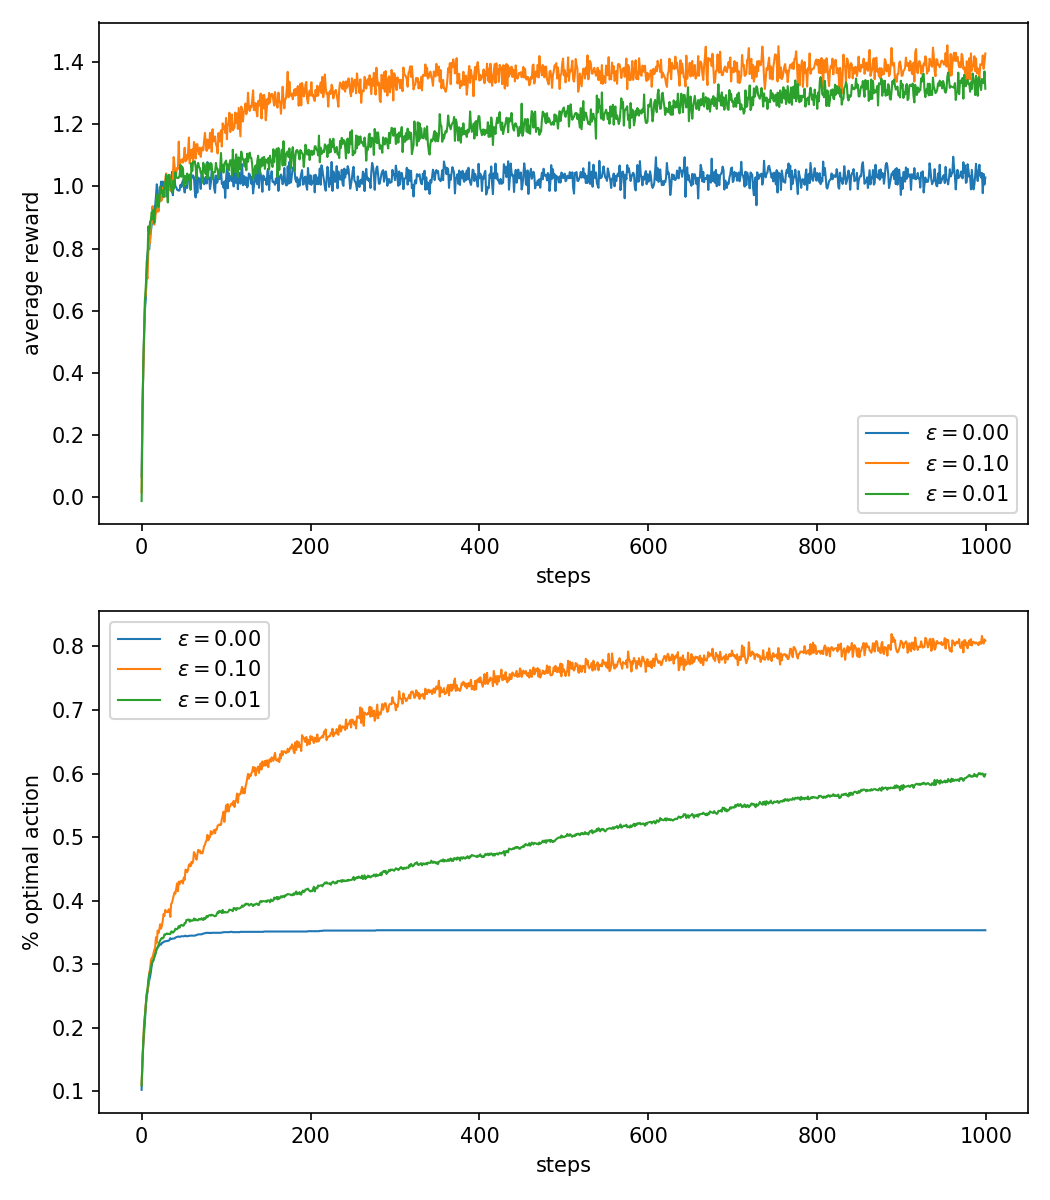
\includegraphics[width=0.85\linewidth]{./figures/chapter2/bandit_testbed.png}
  \captionof{figure}{Comparison of $\varepsilon$-greedy policies on the 10-armed testbed, averaged over 2000 randomly generated problems, each played for 1000 steps.}
  \label{fig:testbed}
\end{center}
The best value of $\varepsilon$ depends on the problem: with noisier rewards more exploration would help, and in longer runs $\varepsilon=0.01$ eventually outperforms $\varepsilon=0.1$.
\end{esempio} 

\begin{algobox}{A simple bandit algorithm}
Initialize, for $a = 1$ to $k$:\\
\hspace*{1.5em}$Q(a) \leftarrow 0$\\
\hspace*{1.5em}$N(a) \leftarrow 0$

\medskip
Loop forever:\\
\hspace*{1.5em}$A \leftarrow
\begin{cases}
  \argmax_a Q(a) & \text{with probability } 1-\varepsilon \\
  \text{a random action} & \text{with probability } \varepsilon
\end{cases}$\\[2pt]
\hspace*{1.5em}$R \leftarrow \mathit{bandit}(A)$\\
\hspace*{1.5em}$N(A) \leftarrow N(A) + 1$\\
\hspace*{1.5em}$Q(A) \leftarrow Q(A) + \frac{1}{N(A)}\bigl[R - Q(A)\bigr]$
\end{algobox}

\subsubsection{Greedy with Optimistic Initialization}
We can initialize the action-value estimates to a high value, this will encourage exploration in the early stages of learning (`optimism in the face of uncertainty'): whatever action is selected, the reward is lower than the estimate, so the agent is `disappointed' and tries the other actions.
The only difference in the algorithm is the initialization of the action-value estimates, which are set to a high value instead of zero ($Q(a)\leftarrow Q_0$). However, it has some limitations:
\begin{itemize}
    \item it only drives early exploration, so it is not well-suited for non-stationary problems;
    \item in some applications we may not know what an optimistic initial value should be.
\end{itemize}
Anyway, it is a convenient heuristic, typically combined with other approaches (e.g., optimistic initialization + $\varepsilon$-greedy).

\subsubsection{Upper-Confidence-Bound (UCB)}
\textit{UCB} uses uncertainty in the value estimates to balance exploration and exploitation. The action selection is based on the following formula:
\[A_t\doteq\argmax_a \left[Q_t(a) + c\sqrt{\frac{\ln t}{N_t(a)}}\right]\]
where $N_t(a)$ is the number of times action $a$ has been selected prior to time $t$ (if $N_t(a)=0$, $a$ is considered a maximizing action). The exploration term comes from \textit{Hoeffding's inequality}. Note that the confidence interval is on our estimate $Q_t(a)$, not on the reward distribution. The more we take an action, the narrower the confidence interval becomes, and the less we explore that action. The parameter $c$ controls the degree of exploration. In a sense, we take the action that potentially could be the best, considering both the estimated value and the uncertainty in that estimate.
\begin{figure}[H]
  \centering
  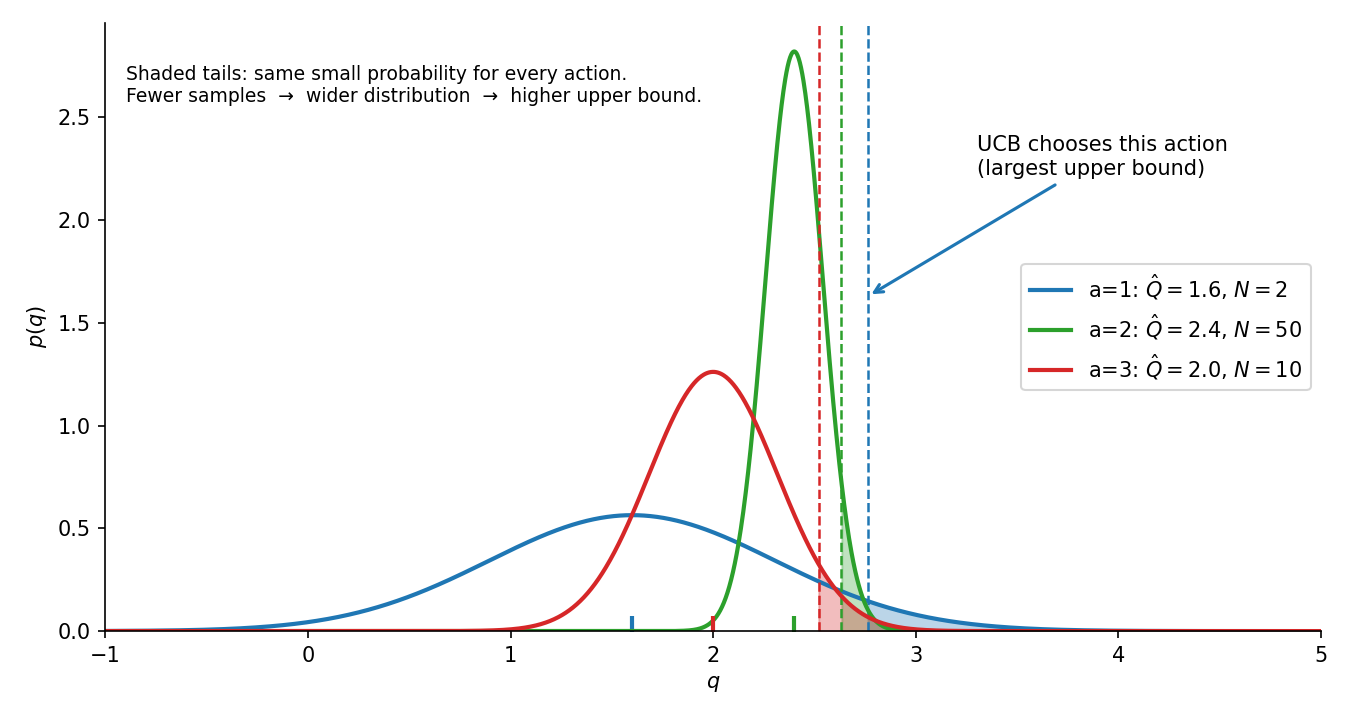
\includegraphics[width=0.9\textwidth]{figures/chapter2/hoeffding_ucb.png}
  \caption{Intuition behind UCB via Hoeffding's inequality. Each curve represents
  the uncertainty about $q_*(a)$; the dashed lines are the upper bounds
  $Q_t(a) + U_t(a)$, chosen so that the shaded tails have the same small
  probability. The least explored action ($N=2$) has the largest bound and is
  selected.}
  \label{fig:hoeffding-ucb}
\end{figure}

\subsubsection{Gradient Bandit Algorithms (GBA)}
In \textit{GBA} a preference for each action is defined $H_t(a)\in\R$, the larger the preference, the more often the action is taken. Preferences have no interpretation in terms of reward: only the relative preference of one action over another matters. The action selection is based on a softmax distribution:
\[\Pr\{A_t=a\}\doteq\frac{e^{H_t(a)}}{\sum_{b=1}^k e^{H_t(b)}}\doteq\pi_t(a)\]
where $\pi_t(a)$ is the probability of taking action $a$ at time $t$. Initially all preferences are equal (e.g., $H_1(a)=0$ for all $a$).
The Gradient Bandit Algorithm updates action preferences using
gradient ascent on the expected reward:

\[
H_{t+1}(a) = H_t(a) +
\alpha (R_t - \bar{R}_t)
\frac{\partial \ln \pi_t(A_t)}{\partial H_t(a)}
\]

Given the softmax policy:

\[
\pi_t(a) =
\frac{e^{H_t(a)}}{\sum_{b=1}^{k} e^{H_t(b)}}
\]

Taking its logarithm:

\[
\ln \pi_t(A_t)
= H_t(A_t) -
\ln \left( \sum_{b=1}^{k} e^{H_t(b)} \right)
\]

The derivative depends on whether the action is selected:

\[
\frac{\partial \ln \pi_t(A_t)}{\partial H_t(a)}
=
\begin{cases}
1 - \pi_t(A_t), & a = A_t \\[4pt]
-\pi_t(a), & a \neq A_t
\end{cases}
\]

that is, $\frac{\partial \ln \pi_t(A_t)}{\partial H_t(a)}=\mathds{1}_{a=A_t}-\pi_t(a)$. Therefore, the two update rules follow directly from
the gradient of the log-softmax policy (the full derivation as stochastic gradient ascent is in the book and is not exam material):

\[H_{t+1}(A_t)\doteq H_t(A_t)+\alpha(R_t-\bar{R}_t)(1-\pi_t(A_t))\]
and for all $a\ne A_t$:
\[H_{t+1}(a)\doteq H_t(a)-\alpha(R_t-\bar{R}_t)\pi_t(a)\]
with $\alpha$ the step-size parameter and $\bar{R}_t$ the average of the rewards up to but not including time $t$, which works as a \textit{baseline}. The update rule increases the preference for the selected action if the received reward is greater than the average reward, and decreases it otherwise.
Higher $\alpha$ causes faster updates, making the policy more deterministic (more Exploitation). A low $\alpha$ causes slower updates, making the policy more stochastic (more Exploration).

\subsection{Summary: comparing exploration strategies}

To compare the methods, each algorithm was run on the 10-armed testbed
for different values of its own parameter, measuring the average reward
over the first 1000 steps (\cref{fig:parameter-study}).

\begin{figure}[H]
  \centering
  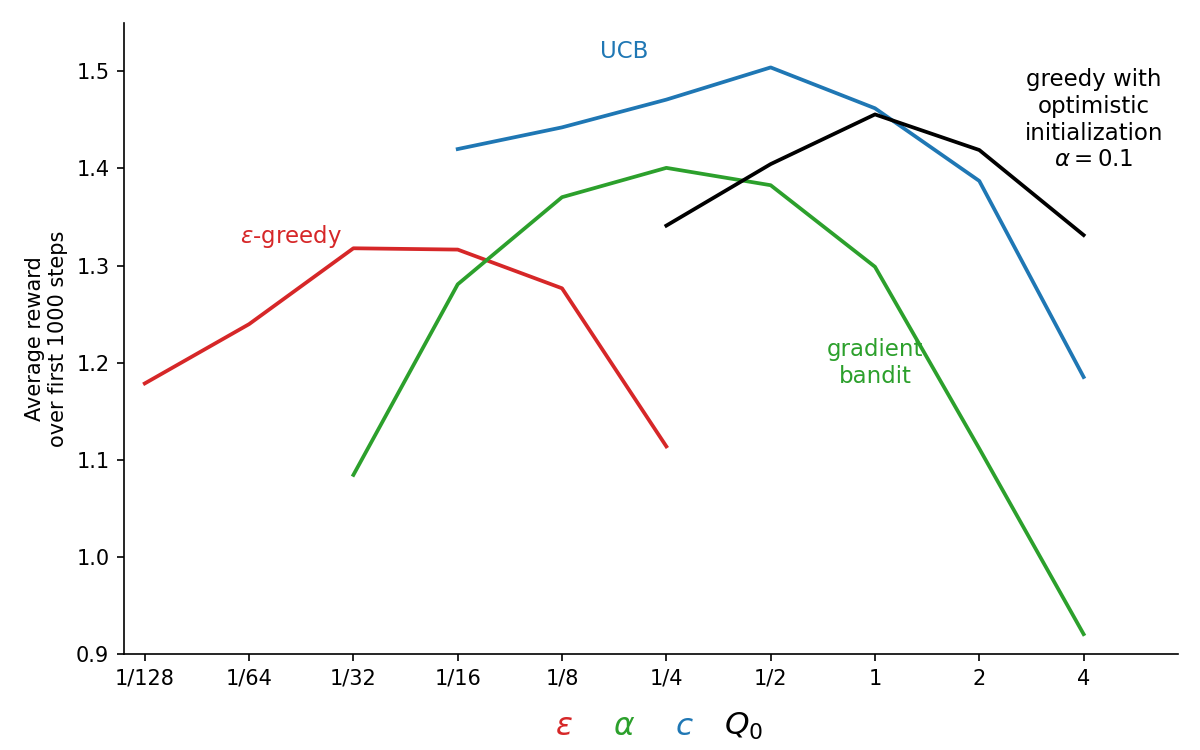
\includegraphics[width=0.85\textwidth]{figures/chapter2/parameter_study.png}
  \caption{Parameter study on the 10-armed testbed: average reward over the first 1000 steps of each algorithm, as a function of its parameter ($\varepsilon$, $\alpha$, $c$ or $Q_0$).}
  \label{fig:parameter-study}
\end{figure}
There is always a trade-off in the choice of the parameter, related to the exploration--exploitation trade-off. The result depends on the problem and on the number of steps
available: with a different horizon, or a non-stationary
problem, the ranking and the best parameters may change a lot.

Topics not covered here: the concept of \textit{regret} (the missed opportunity with respect to always playing the best action) and \textit{contextual bandits} (bandits with states, e.g., using information about the user in advertising).

\section{What Really Matters: Rewards, Not Estimates}
In RL we do not try to model the full reward distributions: it would be too
data-expensive and unnecessary, since our goal is only to maximize the reward
(\emph{``All models are wrong, but some are useful''}, G.~Box). For the same reason, we do not need our estimates $Q(a)$ to be close to the
true values $q_*(a)$. What matters is that they lead us to choose the right
action. A policy is evaluated by the rewards it collects, not by how accurate
its estimates are: estimates that are far from the true values, but still
identify the best action are more useful than estimates that are closer on
average but point to the wrong action.

% !TEX root = ../main.tex
\chapter{MDPs and Bellman Equations}

\section{The story so far ...}
With multiharmed bandits, we have not yet reached a real RL scenario:
\begin{itemize}
    \item The state is always the same, the same action is always optimal;
    \item A single action does not influence future rewards and states.
\end{itemize}

In a real RL scenario, \textit{Markov Decision Processes (MDPs)} describes the environment for Reinforcement Learning.

\section{Markov Processes}
A state $s_t$ is \textit{Markov} if and only if: 
\[P[S_{t+1}|S_t]=P[S_{t+1}|S_1,\cdots,S_t]\]
In Markov processes, we don't have rewards and actions, so the agent has no agency in this case. \textit{State transiction matrix} $\mathcal{P}$ defines the transition probabilities between all states in the environment.
\[
  \mathcal{P} = \textit{from}\;
  \overset{\textstyle\textit{to}}{
  \begin{bmatrix}
    \mathcal{P}_{11} & \dots & \mathcal{P}_{1n} \\
    \vdots           &       &                  \\
    \mathcal{P}_{n1} & \dots & \mathcal{P}_{nn}
  \end{bmatrix}}
\]

\begin{defbox}{Markov Process}
A Markov Process (or \textit{Markov Chain}) is a tuple $\langle \mathcal{S}, \mathcal{P} \rangle$ such that:
\begin{itemize}
    \item $\mathcal{S}$ is a finite set of states;
    \item $\mathcal{P}$ is a state transition probability matrix with entries \[\mathcal{P}_{s,s'} = P[S_{t+1}=s'|S_t=s]\]
        
\end{itemize}
We will always consider finite cases when dealing with episodic tasks.
\end{defbox}

\section{Markov Reward Processes}
\textit{Markov Reward Processes} are Markov chains with reward values.
\begin{defbox}{Markov Reward Process}
A \textit{Markov Reward Process} is a tuple $\langle \mathcal{S}, \mathcal{P}, \mathcal{R}, \gamma \rangle$ such that:
\begin{itemize}
    \item $\mathcal{S}$ is a finite set of states;
    \item $\mathcal{P}$ is a state transition probability matrix with entries \[\mathcal{P}_{s,s'} = P[S_{t+1}=s'|S_t=s]\]
    \item $\mathcal{R}$ is a reward function, $\mathcal{R}_s=\mathbb{E}[R_{t+1}|S_t=s]$;
    \item $\gamma$ is the discount factor, $\gamma\in[0, 1]$.
\end{itemize}
\end{defbox}

\begin{defbox}{}
    The Return $G_t$ is the total discounted reward from time-step $t$:
    \[G_t \doteq R_{t+1} + \gamma R_{t+2} + \cdots = \sum_{k=0}^{\infty} \gamma^k R_{t+k+1}\]
    where $\gamma$ is a discount factor, $\gamma\in[0, 1]$ (0=miopic, 1=far-sighted)
\end{defbox}

The discount is the present value of future rewards.

\begin{defbox}{State Value Function}
    The \textit{state value function} $v(s)$ of a Markov Reward Process is the expected return starting from state $s$:
    \[v(s)=\mathbb{E}[G_t|S_t=s]\]
\end{defbox}

\subsection{Bellman Equation}
We can exploit $G_t$ as follows:
\begin{equation}
\begin{split}
  G_t &\doteq R_{t+1} + \gamma R_{t+2} + \gamma^2 R_{t+3} + \cdots \\
      &= R_{t+1} + \gamma \left( R_{t+2} + \gamma R_{t+3} + \cdots \right) \\
      &= R_{t+1} + \gamma G_{t+1}
\end{split}
\end{equation}
so we have that: 
\begin{equation}
    \begin{split}
        v(s) &= \mathbb{E}[G_t|S_t=s] = \mathbb{E}[R_{t+1} + \gamma G_{t+1}] \\
        &= \mathbb{E}[R_{t+1}+\gamma v(S_{t+1})|S_t=s]
    \end{split}
\end{equation}

We need to consider all possible successor states with the related transition probabilities (real value of $v(s)$, empirical):
\[\mathrm{v}=\mathcal{R}_s+ \gamma \sum_{s'\in S}^{}\mathcal{P}_{ss'}\mathrm{v}(s')\]
The Bellman equation can be written concisely in matrix form:
\[
  \mathrm{v} = \mathcal{R} + \gamma \mathcal{P} \mathrm{v}
\]
where $\mathrm{v}$ is a column vector with one entry per state:
\[
  \begin{bmatrix} \mathrm{v}(1) \\ \vdots \\ \mathrm{v}(n) \end{bmatrix}
  =
  \begin{bmatrix} \mathcal{R}_1 \\ \vdots \\ \mathcal{R}_n \end{bmatrix}
  + \gamma
  \begin{bmatrix}
    \mathcal{P}_{11} & \dots & \mathcal{P}_{1n} \\
    \vdots           &       &                  \\
    \mathcal{P}_{n1} & \dots & \mathcal{P}_{nn}
  \end{bmatrix}
  \begin{bmatrix} \mathrm{v}(1) \\ \vdots \\ \mathrm{v}(n) \end{bmatrix}
\]
so this is a linear system of equations that can be solved in closed form:
\[\mathrm{v}=\mathcal{R}+\gamma \mathcal{P}\mathrm{v}\]
\[(I-\gamma\mathcal{P})\mathrm{v}=\mathcal{R}\]
\[\mathrm{v}=(I-\gamma\mathcal{P})^{-1}\mathcal{R}\]
if we have $n$ states, the cost is $O(n^3)$, affordable only for small Markov Reward Processes. For large MRPs we will look for efficient methods (Dynamic Programming, Monte Carlo evaluation, Temporal Difference Learning).

\subsection{Markov Decision Processes}
A Markov Decision Process (MDP) is a Markov Reward Process with decisions. The agent can choose an action that influences the next state and the reward.
\begin{defbox}{Markov Decision Process}
    A Markov Decision Process is a tuple $\langle \mathcal{S}, \mathcal{A}, \mathcal{P}, \mathcal{R}, \gamma \rangle$ such that:
    \begin{itemize}
        \item $\mathcal{S}$ is a finite set of states;
        \item $\mathcal{A}$ is a finite set of actions;
        \item $\mathcal{P}$ is a state transition probability matrix with entries \[\mathcal{P}_{ss'}^a = P[S_{t+1}=s'|S_t=s, A_t=a]\]
        \item $\mathcal{R}$ is a reward function, $\mathcal{R}_s^a=\mathbb{E}[R_{t+1}|S_t=s, A_t=a]$;
        \item $\gamma$ is the discount factor, $\gamma\in[0, 1]$.
    \end{itemize}
\end{defbox}
Now there is control and agency, whe should define a policy and we can try to maximize the reward.
\begin{definition}[Policy]
    A policy $\pi$ is a distribution over actions given that we are in a state:
    \[\pi(a|s)=P[A_t=a|S_t=s]\]
\end{definition}
The policy fully defines the agent's behavior. In MDP policies are stationary (independent of $t$). Moreover we consider stochastic policies, that is, the agent can choose an action with a certain probability, this allow us to deal with exploration.

Given an MDP $\langle \mathcal{S}, \mathcal{A}, \mathcal{P}, \mathcal{R}, \gamma \rangle$ and a policy $\pi$:
\begin{itemize}
    \item The state sequence $S_0, S_1, S_2, \ldots$ is a Markov Process where: \\ \[\mathcal{P}_{ss'}^\pi=\sum_{a\in\mathcal{A}}\pi(a|s)\mathcal{P}_{ss'}^a\]
    \item The state and reward sequence $S_0, R_1, S_1, R_2, S_2, R_3, \ldots$ is a Markov Reward Process where: \\ \[\mathcal{R}_s^\pi=\sum_{a\in\mathcal{A}}\pi(a|s)\mathcal{R}_s^a\] 
\end{itemize}

Now we can define the value function, and also a q-value function, for a policy $\pi$:
\begin{defbox}{State Value Function for a Policy}
    The \textit{state value function} $v_\pi(s)$ of a Markov Decision Process is the expected return starting from state $s$ and following policy $\pi$:
    \[v_\pi(s)=\mathbb{E}_\pi[G_t|S_t=s]\]
\end{defbox}
\begin{defbox}{Action Value Function for a Policy}
    The \textit{action value function} $q_\pi(s, a)$ of a Markov Decision Process is the expected return starting from state $s$, taking action $a$ and following policy $\pi$:
    \[q_\pi(s, a)=\mathbb{E}_\pi[G_t|S_t=s, A_t=a]\]
\end{defbox}

\subsection{Bellaman Expectation Equation}
The value function $v_{\pi}(s)$ can, again, be decomposed as before:
\[v_\pi(s) = \mathbb{E}_\pi[R_{t+1} + \gamma v_\pi(S_{t+1}) | S_t = s]\]
similarly for the action value function:
\[q_\pi(s, a) = \mathbb{E}_\pi[R_{t+1} + \gamma q_\pi(S_{t+1}, A_{t+1}) | S_t = s, A_t = a]\]
We can define the true values for value and action-value functions as follows:
\[\mathrm{v}_\pi(s)=\sum_{a\in A}^{}\pi(a|s)\mathrm{q}_\pi(s,a)\]
\[\mathrm{q}_\pi(s,a)=\mathcal{R}_s^a+\gamma\sum_{s'\in S}\mathcal{P}_{ss'}^a\mathrm{v}_\pi(s')\]
and we can obtain recursive description of $\mathrm{v}$:
\[\mathrm{v}_\pi(s)=\sum_{a\in A}^{}\pi(a|s)\left(\mathcal{R}_s^a+\gamma\sum_{s'\in S}\mathcal{P}_{ss'}^a\mathrm{v}_\pi(s')\right)\]
and also for $\mathrm{q}$:
\[\mathrm{q}_\pi(s,a)=\mathcal{R}_s^a+\gamma\sum_{s'\in S}\mathcal{P}_{ss'}^a\sum_{a'\in A}\pi(a'|s')\mathrm{q}_\pi(s',a')\]
Also Bellman Expectation Equations can be written in matrix form:
\[\mathrm{v}_\pi=\mathcal{R}^\pi+\gamma\mathcal{P}^\pi\mathrm{v}_\pi\]
\[\mathrm{v}_\pi=(I-\gamma\mathcal{P}^\pi)^{-1}\mathcal{R}^\pi\]

% !TEX root = ../main.tex
\chapter{Bellman Optimality Equations and DP}

\section{Optimal Value Functions and Optimal Policy}
The \textit{optimal state-value function} $v_*(s)$ is the maximum state-value function over all policies, and the \textit{optimal action-value function} $q_*(s,a)$ is the maximum action-value function over all policies:
\[v_*(s)=\max_\pi v_\pi(s)\qquad q_*(s,a)=\max_\pi q_\pi(s,a)\]
An MDP can be considered `solved' when $q_*$ is known: we always know the optimal action to take in each state. (Notation: a $*$ always denotes optimality.)

We can define an order over policies: $\pi\geq\pi'$ if $v_\pi(s)\geq v_{\pi'}(s)$ for all $s\in\mathcal{S}$.
\begin{theorem}
    For any finite MDP ($\mathcal{S},\mathcal{A}, \mathcal{R}$ finite sets):
    \begin{enumerate}
        \item There exists an optimal policy $\pi_*$ such that $\pi_*\geq\pi$ for all possible $\pi$;
        \item All optimal policies achieve the optimal state-value function \[v_{\pi_*}(s)=v_*(s)\]
        \item All optimal policies achieve the optimal action-value function \[q_{\pi_*}(s,a)=q_*(s,a)\]
    \end{enumerate}
\end{theorem}
Intuitively, given two policies we can build a new one that, in each state, follows the policy with the higher value in that state: it is at least as good as both. In a finite MDP, repeating this yields a policy that is at least as good as all the others.

A simple approach to find the optimal policy, if we have $q_*(s,a)$, is to maximize over the actions:
\[
  \pi_*(a \mid s) =
  \begin{dcases}
    1 & \text{if } a = \argmax_{a \in \mathcal{A}} q_*(s, a) \\
    0 & \textit{otherwise}
  \end{dcases}
\]
So there is always a deterministic optimal policy for any MDP. But how do we get $q_*$?

\section{Bellman Optimality Equation}
The Bellman Optimality Equation (not to be confused with the Bellman Expectation Equation, which holds for a generic policy) defines $v_*$ recursively with itself, again with a 1-step look-ahead:
\begin{figure}[H]
\centering
\tikzset{
  state/.style={circle, draw, thick, minimum size=7mm, inner sep=0pt},
  action/.style={circle, fill, minimum size=3mm, inner sep=0pt}
}
\begin{subfigure}[t]{0.48\textwidth}
  \centering
  \begin{tikzpicture}
    \node[state]  (s)  at (0, 0)     {};
    \node[action] (a1) at (-1.3, -2) {};
    \node[action] (a2) at ( 1.3, -2) {};
    \draw[thick] (s) -- (a1);
    \draw[thick] (s) -- (a2);
    \draw[thick] (0,0) ++(237:1.15) arc (237:303:1.15); % max
    \node[left=4mm of s]  {$v_*(s) \mapsfrom s$};
    \node[left=2mm of a1] {$q_*(s,a) \mapsfrom a$};
  \end{tikzpicture}
  \caption{The arc indicates the max over all possible choices of the
  action value: we don't need to average.}
  \label{fig:backup-vstar}
\end{subfigure}
\hfill
\begin{subfigure}[t]{0.48\textwidth}
  \centering
  \begin{tikzpicture}
    \node[action] (sa) at (0, 0)     {};
    \node[state]  (s1) at (-1.3, -2) {};
    \node[state]  (s2) at ( 1.3, -2) {};
    \draw[thick] (sa) -- (s1) node[midway, left=2mm] {$r$};
    \draw[thick] (sa) -- (s2);
    \node[left=2mm of sa] {$q_*(s,a) \mapsfrom s,a$};
    \node[left=2mm of s1] {$v_*(s') \mapsfrom s'$};
  \end{tikzpicture}
  \caption{Here we need to average over the possible successor states
  and rewards.}
  \label{fig:backup-qstar}
\end{subfigure}
\caption{Backup diagrams for $v_*$ and $q_*$.}
\label{fig:backup-optimal}
\end{figure}
\[\mathrm{v}_*(s)=\max_a\mathrm{q}_*(s,a)\qquad \mathrm{q}_*(s,a)=\mathcal{R}_s^a+\gamma\sum_{s'\in\mathcal{S}}\mathcal{P}_{ss'}^a\,\mathrm{v}_*(s')\]
so, if we plug one into the other we obtain:
\[\mathrm{v}_*(s)=\max_a\left(\mathcal{R}_s^a+\gamma\sum_{s'\in\mathcal{S}}\mathcal{P}_{ss'}^a\,\mathrm{v}_*(s')\right)\]
\[\mathrm{q}_*(s,a)=\mathcal{R}_s^a+\gamma\sum_{s'\in\mathcal{S}}\mathcal{P}_{ss'}^a\max_{a'}\mathrm{q}_*(s',a')\]
Since there is a non-linear operation (max) we don't have a closed-form solution, and we need iterative methods (value iteration, policy iteration, Q-learning, SARSA, \dots).

\begin{table}[H]
\centering
\begin{tabular}{@{}l l p{4.2cm}@{}}
\toprule
\textbf{Equation} & \textbf{Used for} & \textbf{Solution} \\
\midrule
MRP Bellman equation & $v$ & linear: closed form for small MRPs \\
MDP Bellman expectation equation & $v_\pi$, $q_\pi$ & linear: closed form for small MDPs \\
MDP Bellman optimality equation & $v_*$, $q_*$ & non-linear: iterative methods \\
\bottomrule
\end{tabular}
\caption{The three Bellman equations.}
\label{tab:bellman-eqs}
\end{table}

\section{Dynamic Programming for MDPs}
In real Reinforcement Learning problems we don't have access to $\mathcal{P}$ and $\mathcal{R}$, but in this chapter we assume that the MDP is fully known (this is a strong assumption, called the \textit{planning} problem).
Our goal is to solve the Markov Decision Process:
\begin{itemize}
    \item Policy Evaluation: given a policy $\pi$ we want to derive the value function $v_\pi$ and $q_\pi$;
    \item Policy improvement (control): improve the current policy $\pi$ to a better one $\pi'$, in order to find the optimal policy $\pi_*$ typically deriving $v_*$ and $q_*$;
\end{itemize}
There can be multiple optimal policies, but they all achieve the same optimal value function $v_*$ and $q_*$.

Even if $\mathcal{P}$ and $\mathcal{R}$ are known, solving the MDP may not be straightforward: prediction could be solved with a set of linear equations, but this is too expensive for large MDPs, and control requires the non-linear Bellman Optimality Equation. Dynamic Programming solves both by using the Bellman equations as iterative update rules for our estimates, until they converge.

The idea of Dynamic Programming is to break complex problems into simpler subproblems and solve them recursively. Then we combine the solutions to the subproblems for solving the original one.
DP is a tool that allows us to solve problems with these two properties:
\begin{itemize}
    \item \textit{optimal substructure}: an optimal solution can be decomposed into optimal solutions of subproblems (principle of optimality);
    \item \textit{overlapping subproblems}: subproblems recur many times, so their solutions can be cached and reused.
\end{itemize}
MDPs satisfy both properties, thanks to the recursive structure of the Bellman equations.

\subsection{Prediction: Policy Evaluation}
\begin{equation}
  \begin{split}
    v_\pi(s) &\doteq \mathbb{E}_\pi[G_t \mid S_t=s] \\
      &= \mathbb{E}_\pi[R_{t+1}+\gamma G_{t+1} \mid S_t=s] \\
      &= \mathbb{E}_\pi[R_{t+1}+\gamma v_\pi(S_{t+1}) \mid S_t=s] \\
      &= \sum_{a}\pi(a|s)\sum_{s',r}p(s',r|s,a)\bigl[r+\gamma v_\pi(s')\bigr]
  \end{split}
\end{equation}
Instead of solving the Bellman equation directly we can use it as an update rule (for all $s\in\mathcal{S}$):
\begin{equation}
  v_{k+1}(s) \doteq \sum_{a}\pi(a|s)\sum_{s',r}p(s',r|s,a)\bigl[r+\gamma v_k(s')\bigr]
\end{equation}
The dynamic programming procedure starts from an initial guess of $v$ that is iteratively improved by repeatedly applying the Bellman Expectation Equation. $v_k=v_\pi$ is a fixed point of this update, and the sequence $\{v_k\}$ converges to $v_\pi$ as $k\to\infty$.

\emph{Synchronous} policy evaluation stores two copies of the value
function, for all states:
\[
  \mathrm{v}_{\text{new}}(s) \leftarrow \sum_{a \in \mathcal{A}}\pi(a\mid s)
  \left( \mathcal{R}_s^a + \gamma \sum_{s' \in \mathcal{S}}
  \mathcal{P}_{ss'}^a \, \mathrm{v}_{\text{old}}(s') \right)
\]
\[
  \mathrm{v}_{\text{old}} \leftarrow \mathrm{v}_{\text{new}}
\]

\emph{In-place} policy evaluation only stores one copy of the value
function:
\[
  \mathrm{v}(s) \leftarrow \sum_{a \in \mathcal{A}}\pi(a\mid s)
  \left( \mathcal{R}_s^a + \gamma \sum_{s' \in \mathcal{S}}
  \mathcal{P}_{ss'}^a \, \mathrm{v}(s') \right)
\]
While synchronous updates seem more rigorous, in-place updates achieve faster convergence, since we use the new estimates as soon as they are available. In practice we will typically use in-place updates. If we have domain knowledge, a reasonable initialization can also speed up convergence.
\begin{algobox}{Iterative Policy Evaluation (in-place version), for estimating $V \approx \mathrm{v}_\pi$}
Input $\pi$, the policy to be evaluated\\
Algorithm parameter: a small threshold $\theta > 0$ determining accuracy of estimation\\
Initialize $V(s)$, for all $s \in \mathcal{S}^+$, arbitrarily except that
$V(\mathit{terminal}) = 0$

\medskip
Loop:\\
\hspace*{1.5em}$\Delta \leftarrow 0$\\
\hspace*{1.5em}Loop for each $s \in \mathcal{S}$:\\
\hspace*{3em}$v \leftarrow V(s)$\\
\hspace*{3em}$V(s) \leftarrow \sum_a \pi(a \mid s) \sum_{s',r} p(s',r \mid s,a)
  \bigl[r + \gamma V(s')\bigr]$\\
\hspace*{3em}$\Delta \leftarrow \max\bigl(\Delta, \lvert v - V(s) \rvert\bigr)$\\
until $\Delta < \theta$
\end{algobox}

\subsection{Control: Policy Improvement}
One way to improve a policy is to evaluate it and then improve it by acting greedily with respect to $v_\pi$:
\[\pi'=\text{greedy}(\mathrm{v}_\pi),\qquad \pi'(s)=\argmax_a q_\pi(s,a)=\argmax_a\left(\mathcal{R}_s^a+\gamma\sum_{s'}\mathcal{P}_{ss'}^a\mathrm{v}_\pi(s')\right)\]
We can evaluate $v_{\pi'}$ and then improve the policy again. This procedure, called \textit{policy iteration}, proceeds until the policy converges to the optimal policy $\pi_*$, with $v_{\pi_*}=v_*$.
We will show that acting greedily can improve the policy and allow us to reach optimality.

\begin{algobox}{Policy Iteration (using iterative policy evaluation) for estimating $\pi \approx \pi_*$}
1. Initialization\\
\hspace*{1.5em}$V(s) \in \mathbb{R}$ and $\pi(s) \in \mathcal{A}(s)$ arbitrarily for all $s \in \mathcal{S}$

\medskip
2. Policy Evaluation\\
\hspace*{1.5em}Loop:\\
\hspace*{3em}$\Delta \leftarrow 0$\\
\hspace*{3em}Loop for each $s \in \mathcal{S}$:\\
\hspace*{4.5em}$v \leftarrow V(s)$\\
\hspace*{4.5em}$V(s) \leftarrow \sum_{s',r} p(s',r \mid s,\pi(s))\bigl[r + \gamma V(s')\bigr]$\\
\hspace*{4.5em}$\Delta \leftarrow \max\bigl(\Delta, \lvert v - V(s) \rvert\bigr)$\\
\hspace*{1.5em}until $\Delta < \theta$ (a small positive number determining the accuracy of estimation)

\medskip
3. Policy Improvement\\
\hspace*{1.5em}$\mathit{policy\text{-}stable} \leftarrow \mathit{true}$\\
\hspace*{1.5em}For each $s \in \mathcal{S}$:\\
\hspace*{3em}$\mathit{old\text{-}action} \leftarrow \pi(s)$\\
\hspace*{3em}$\pi(s) \leftarrow \argmax_a \sum_{s',r} p(s',r \mid s,a)\bigl[r + \gamma V(s')\bigr]$\\
\hspace*{3em}If $\mathit{old\text{-}action} \neq \pi(s)$, then $\mathit{policy\text{-}stable} \leftarrow \mathit{false}$\\
\hspace*{1.5em}If $\mathit{policy\text{-}stable}$, then stop and return $V \approx \mathrm{v}_*$ and $\pi \approx \pi_*$; else go to 2
\end{algobox}

\begin{figure}[H]
\centering
\begin{tikzpicture}[>={Stealth[length=2.6mm]}]
  \coordinate (P) at (10,0);
  \def\k{0.28}

  % the two lines
  \draw[thick] (0,{\k*10})  -- (P);
  \draw[thick] (0,{-\k*10}) -- (P);

  % zig-zag between the two lines
  \draw[->, thick] (1.2, {\k*8.8})  -- (2.9, {-\k*7.1});
  \draw[->, thick] (2.9, {-\k*7.1}) -- (4.7, {\k*5.3});
  \draw[->, thick] (4.7, {\k*5.3})  -- (6.0, {-\k*4.0});
  \draw[->, thick] (6.0, {-\k*4.0}) -- (7.1, {\k*2.9});
  \draw[->, thick] (7.1, {\k*2.9})  -- (7.9, {-\k*2.1});
  \draw[->, thick] (7.9, {-\k*2.1}) -- (8.5, {\k*1.5});
  \draw[->, thick] (8.5, {\k*1.5})  -- (8.9, {-\k*1.1});
  \draw[->, thick] (8.9, {-\k*1.1}) -- (9.2, {\k*0.8});

  % starting point
  \node[left, align=center] (start) at (-0.3, 0.2) {starting\\ $V$\;$\pi$};
  \draw[->, thick] (start.east |- 0,0.5) -- (1.2, {\k*8.8});

  % limit point and labels
  \fill (P) circle (1.8pt);
  \node[right, align=center] at (10.1, 0) {$\mathrm{v}_*$\\ $\pi_*$};
  \node[above, rotate=-15.6, font=\small] at (3.0, {\k*7.0}) {$V = \mathrm{v}_\pi$};
  \node[below, rotate=15.6, font=\small] at (4.5, {-\k*5.5}) {$\pi = \text{greedy}(V)$};
\end{tikzpicture}
\caption{Policy iteration: evaluation ($V=\mathrm{v}_\pi$) and greedy improvement ($\pi=\text{greedy}(V)$) alternate until they converge to $\mathrm{v}_*$ and $\pi_*$.}
\label{fig:policy-iteration}
\end{figure}

\begin{theorem}[Policy Improvement Theorem]
    Let's consider a deterministic policy $\pi$. We can improve the policy by acting greedily:
    \[\pi'(s)=\argmax_{a\in\mathcal{A}}q_\pi(s,a)\]
    that is, we pick the action that provides the best value and then we follow $\pi$. Then the new policy $\pi'$ is better than or equal to the old one $\pi$:
    \[q_\pi(s,\pi'(s))=\max_{a\in\mathcal{A}}q_\pi(s,a)\geq q_\pi(s,\pi(s))=\mathrm{v}_\pi(s)\]
    A policy $\pi'\geq\pi$ if $\mathrm{v}_{\pi'}(s)\geq\mathrm{v}_\pi(s)$ for all $s\in\mathcal{S}$. This improves the whole value function:
    \begin{equation}
      \begin{split}
        \mathrm{v}_\pi(s)\leq q_\pi(s,\pi'(s))&=\mathbb{E}_{\pi'}[R_{t+1}+\gamma \mathrm{v}_\pi(S_{t+1})\mid S_t=s]\\
        &\leq \mathbb{E}_{\pi'}[R_{t+1}+\gamma q_\pi(S_{t+1},\pi'(S_{t+1}))\mid S_t=s]\\
        &\leq \mathbb{E}_{\pi'}[R_{t+1}+\gamma R_{t+2}+\gamma^2q_\pi(S_{t+2},\pi'(S_{t+2}))\mid S_t=s]\\
        &\leq \mathbb{E}_{\pi'}[R_{t+1}+\gamma R_{t+2}+\gamma^2R_{t+3}+\cdots\mid S_t=s]\\
        &=\mathrm{v}_{\pi'}(s)
      \end{split}
    \end{equation}
    Now we are sure that by acting greedily we are not going to do worse, but we still have to prove that we reach optimality. Let's consider the case in which improvement stops:
    \[q_\pi(s,\pi'(s))=\max_{a\in\mathcal{A}}q_\pi(s,a)=q_\pi(s,\pi(s))=\mathrm{v}_\pi(s)\]
    In this case we have satisfied the Bellman Optimality Equation:
    \[\mathrm{v}_\pi(s)=\max_{a\in\mathcal{A}}q_\pi(s,a)\]
    Therefore we have reached optimality and $\pi$ is an optimal policy:
    \[\mathrm{v}_\pi(s)=\mathrm{v}_*(s)\quad\text{for all } s\in\mathcal{S}.\]
    Policy iteration actually solves MDPs.
\end{theorem}

\subsection{Control: Value Iteration}
Policy evaluation can be slow, and we do not need the exact value of $v_\pi$: the evaluation step can be truncated without losing the convergence guarantees. In \textit{value iteration} the evaluation step is stopped after a single update. The approach can be written as:
\begin{equation}
  \begin{split}
    v_{k+1}(s)&\doteq\max_a\mathbb{E}\left[R_{t+1}+\gamma v_k(S_{t+1})\mid S_t=s,A_t=a\right]\\
    &=\max_a\sum_{s',r}^{}p(s',r|s,a)\left[r+\gamma v_k(s')\right]
  \end{split}
\end{equation}
for all $s\in\mathcal{S}$. We are combining policy evaluation and policy improvement in a single step. It can be shown that this approach converges to the optimal value function $v_*$, and then we can derive the optimal policy $\pi_*$ by acting greedily with respect to $v_*$.
The main difference with policy evaluation is that here we use the Bellman Optimality Equation instead of the Bellman Expectation Equation:
instead of averaging over all actions, we just consider the best one. No policy is needed during the iterations, and value iteration also works for continuing problems (no terminal states), provided that $\gamma<1$.
\begin{algobox}{Value Iteration, for estimating $\pi \approx \pi_*$}
Algorithm parameter: a small threshold $\theta > 0$ determining accuracy of estimation\\
Initialize $V(s)$, for all $s \in \mathcal{S}^+$, arbitrarily except that
$V(\mathit{terminal}) = 0$

\medskip
Loop:\\
\hspace*{1.5em}$\Delta \leftarrow 0$\\
\hspace*{1.5em}Loop for each $s \in \mathcal{S}$:\\
\hspace*{3em}$v \leftarrow V(s)$\\
\hspace*{3em}$V(s) \leftarrow \max_a \sum_{s',r} p(s',r \mid s,a)\bigl[r + \gamma V(s')\bigr]$\\
\hspace*{3em}$\Delta \leftarrow \max\bigl(\Delta, \lvert v - V(s) \rvert\bigr)$\\
until $\Delta < \theta$

\medskip
Output a deterministic policy, $\pi \approx \pi_*$, such that\\
\hspace*{1.5em}$\pi(s) = \argmax_a \sum_{s',r} p(s',r \mid s,a)\bigl[r + \gamma V(s')\bigr]$
\end{algobox}
In this algorithm we are also considering the in-place update of $V$.
\begin{figure}[H]
\centering
\begin{subfigure}[t]{0.48\textwidth}
  \centering
  \begin{tikzpicture}[scale=0.75, >={Stealth[length=2.2mm]}]
    \gpibase
    \tikzset{zig/.style={->, very thick, arrowblue}}
    \draw[zig] (0,0.6)       -- (0.78,2.09);
    \draw[zig] (0.78,2.09)   -- (1.66,-1.0);
    \draw[zig] (1.66,-1.0)   -- (2.8,1.28);
    \draw[zig] (2.8,1.28)    -- (3.38,-0.6);
    \draw[zig] (3.38,-0.6)   -- (4.0,0.8);
    \draw[zig] (4.0,0.8)     -- (4.37,-0.375);
    \draw[zig] (4.37,-0.375) -- (4.78,0.49);
    \draw[zig] (4.78,0.49)   -- (5.04,-0.22);
  \end{tikzpicture}
  \caption{Policy iteration}
\end{subfigure}
\hfill
\begin{subfigure}[t]{0.48\textwidth}
  \centering
  \begin{tikzpicture}[scale=0.75, >={Stealth[length=2.2mm]}]
    \gpibase
    \tikzset{zig/.style={->, very thick, arrowblue}}
    \draw[zig] (0,0.56)     -- (0.72,1.32);
    \draw[zig] (0.72,1.32)  -- (1.6,-0.28);
    \draw[zig] (1.6,-0.28)  -- (2.74,0.80);
    \draw[zig] (2.74,0.80)  -- (3.36,-0.09);
    \draw[zig] (3.36,-0.09) -- (3.88,0.28);
    \draw[zig] (3.88,0.28)  -- (4.29,-0.09);
    \draw[zig] (4.29,-0.09) -- (4.81,0.23);
    \draw[zig] (4.81,0.23)  -- (5.17,-0.08);
  \end{tikzpicture}
  \caption{Value iteration}
\end{subfigure}
\caption{Policy iteration vs.\ value iteration (adapted from A.~White and
M.~White, \emph{Fundamentals of Reinforcement Learning}).
Policy iteration alternates full evaluation and improvement, jumping between
the two lines; value iteration takes smaller, interleaved steps that stay
between them.}
\label{fig:pi-vs-vi}
\end{figure}

\subsection{Generalized Policy Iteration (GPI)}
We may also use hybrid strategies between policy iteration and value iteration. \textit{Generalized Policy Iteration} is the general idea of letting policy evaluation and policy improvement interact, independently of the granularity of the two processes: almost all RL methods can be described as GPI.

\begin{table}[H]
\centering
\begin{tabular}{@{}l p{5.5cm} l@{}}
\toprule
\textbf{Problem} & \textbf{Bellman equation} & \textbf{Algorithm} \\
\midrule
Prediction & Bellman expectation equation & Iterative Policy Evaluation \\
Control    & Bellman expectation equation + Greedy Policy Improvement & Policy Iteration \\
Control    & Bellman optimality equation & Value Iteration \\
\bottomrule
\end{tabular}
\caption{Summary of the (synchronous) DP algorithms. They are based on $v_\pi(s)$ or $v_*(s)$, with complexity $O(mn^2)$ per iteration for $m$ actions and $n$ states; they could also be applied to $q_\pi(s,a)$ or $q_*(s,a)$, with complexity $O(m^2n^2)$ per iteration.}
\label{tab:dp-summary}
\end{table}

\subsection{Asynchronous DP}
All the approaches seen so far are \emph{sweep-based}: each iteration backs up all the states. The same two implementations seen for policy evaluation also hold for value iteration (with the max instead of the expectation over $\pi$): the \emph{synchronous} version stores two copies of the value function,
\[
  \mathrm{v}_{\text{new}}(s) \leftarrow \max_{a \in \mathcal{A}}
  \left( \mathcal{R}_s^a + \gamma \sum_{s' \in \mathcal{S}}
  \mathcal{P}_{ss'}^a \, \mathrm{v}_{\text{old}}(s') \right),
  \qquad
  \mathrm{v}_{\text{old}} \leftarrow \mathrm{v}_{\text{new}},
\]
while the \emph{in-place} version only stores one copy:
\[
  \mathrm{v}(s) \leftarrow \max_{a \in \mathcal{A}}
  \left( \mathcal{R}_s^a + \gamma \sum_{s' \in \mathcal{S}}
  \mathcal{P}_{ss'}^a \, \mathrm{v}(s') \right).
\]
\emph{Asynchronous} DP methods are in-place methods that are not organized in systematic sweeps: they back up states individually, in any order whatsoever, using whatever values of other states happen to be available. This can significantly reduce computation: if the state set is very large, even a single sweep can be prohibitively expensive. Asynchronous DP still converges if all states continue to be selected. Some examples:
\begin{itemize}
    \item select the states to update so as to improve the rate of progress of the algorithm;
    \item skip states that are not relevant to optimal behavior;
    \item collect trajectories and only update the states that are actually visited by the policy;
    \item \emph{prioritized sweeping} (Chapter 8): back up the state with the largest remaining Bellman error, using a priority queue (it requires knowledge of the predecessor states).
\end{itemize}

% !TEX root = ../main.tex
\chapter{Monte Carlo Methods}

\textit{Monte Carlo (MC) Methods} are simple and effective approaches to deal with `full' RL problems (without knowing $\mathcal{P}$ and $\mathcal{R}$). These methods only require experience (sample sequences of states, actions and rewards, i.e., real-world data gathered by interacting with the environment) and episodic tasks. MC is our first \textit{model-free} approach, for both prediction and control.

MC methods estimate expectations by averaging over a large number of random samples. 
Since $v_\pi(s)=\mathbb{E}_\pi[G_t\mid S_t=s]$ and $q_\pi(s,a)=\mathbb{E}_\pi[G_t\mid S_t=s,A_t=a]$ are expectations, we can approximate the true expected returns (state-value and action-value functions) with the average of the returns seen if we collect enough data.

Pay attention! Even if $\mathcal{P}$ and $\mathcal{R}$ are not known, we will not use data to estimate such quantities.
For efficiency, we will resort to \textit{model-free} RL approaches, that will estimate instead $\mathrm{v}$ and $\mathrm{q}$ (later directly $\pi$). There are also \textit{model-based} RL approaches.
\section{Prediction: First-visit MC prediction}
We generate an episode and, going backwards, we update the estimate of each visited state with the return observed after its \emph{first} visit: if $S_t$ already appears at an earlier step of the episode, the update is skipped. Only visited states are updated.

\begin{algobox}{First-visit MC prediction, for estimating $V \approx \mathrm{v}_\pi$}
\raggedright
Input: a policy $\pi$ to be evaluated

\medskip
Initialize:\\
\hspace*{1.5em}$V(s) \in \mathbb{R}$, arbitrarily, for all $s \in \mathcal{S}$\\
\hspace*{1.5em}$\mathit{Returns}(s) \leftarrow$ an empty list, for all $s \in \mathcal{S}$

\medskip
Loop forever (for each episode):\\
\hspace*{1.5em}Generate an episode following $\pi$:\\
\hspace*{3em}$S_0, A_0, R_1, S_1, A_1, R_2, \dots, S_{T-1}, A_{T-1}, R_T$\\
\hspace*{1.5em}$G \leftarrow 0$\\
\hspace*{1.5em}Loop for each step of episode, $t = T-1, T-2, \dots, 0$:\\
\hspace*{3em}$G \leftarrow \gamma G + R_{t+1}$\\
\hspace*{3em}Unless $S_t$ appears in $S_0, S_1, \dots, S_{t-1}$:\\
\hspace*{4.5em}Append $G$ to $\mathit{Returns}(S_t)$\\
\hspace*{4.5em}$V(S_t) \leftarrow \operatorname{average}\bigl(\mathit{Returns}(S_t)\bigr)$
\end{algobox}

The \textit{Every-visit} MC prediction algorithm is similar to the first-visit one, but it updates the value of a state every time it appears in an episode, not just the first time. This means that the same state can be updated multiple times in a single episode. So the difference in the pseudo-code is that the \textit{Unless} condition no longer appears. Instead of storing all the returns, a more efficient implementation uses incremental updates:
\[N(S_t)\leftarrow N(S_t)+1,\qquad V(S_t)\leftarrow V(S_t)+\frac{1}{N(S_t)}\bigl[G_t-V(S_t)\bigr]\]
or, with a constant step-size (better for non-stationary problems), $V(S_t)\leftarrow V(S_t)+\alpha\bigl[G_t-V(S_t)\bigr]$.

Some properties of MC prediction:
\begin{itemize}
    \item MC learns directly from experience: there is no need to keep a model of the environment;
    \item the estimate of each state is independent of the estimates of the other states (MC does not bootstrap, unlike DP);
    \item the computation needed to update each state does not depend on the size of the MDP, but on the length of the episode.
\end{itemize}

The reason why we compute the return of each visited state by going backwards from the final time-step is that it requires fewer computations:

\begin{figure}[H]
\centering
\begin{tikzpicture}[>={Stealth[length=2mm]}, font=\small,
    st/.style={circle, draw, minimum size=5mm, inner sep=0pt},
    term/.style={rectangle, draw, fill=gray!50, minimum size=5mm, inner sep=0pt},
    eq/.style={font=\footnotesize},
    cnt/.style={draw, font=\footnotesize, inner sep=3pt}]

  % chain of states with rewards
  \foreach \i in {0,...,4} { \node[st] (s\i) at (1.5*\i, 0) {}; }
  \node[term] (T) at (7.5, 0) {};
  \foreach \i/\j/\r in {0/1/3, 1/2/4, 2/3/7, 3/4/1} {
    \draw[->, thick] (s\i) -- node[above] {\r} (s\j);
  }
  \draw[->, thick] (s4) -- node[above] {2} (T);
  \node[right=8mm of T] {$\gamma = 0.5$};

  % left: backward recursion (staircase)
  \node[eq, anchor=west] at (0.0, -1.3) {$G_0 = R_1 + \gamma G_1$};
  \node[eq, anchor=west] at (0.6, -2.0) {$G_1 = R_2 + \gamma G_2$};
  \node[eq, anchor=west] at (1.2, -2.7) {$G_2 = R_3 + \gamma G_3$};
  \node[eq, anchor=west] at (1.8, -3.4) {$G_3 = R_4 + \gamma G_4$};
  \node[eq, anchor=west] at (2.4, -4.1) {$G_4 = R_5 + \gamma G_5$};
  \node[eq, anchor=west] at (3.0, -4.8) {$G_5 = 0$};
  \node[cnt] at (2.6, -5.7) {5 additions};

  % right: direct sums, right-aligned
  \node[eq, anchor=east] at (12.3, -1.3) {$G_0 = R_1 + \gamma R_2 + \gamma^2 R_3 + \gamma^3 R_4 + \gamma^4 R_5 = 7$};
  \node[eq, anchor=east] at (12.3, -2.0) {$G_1 = R_2 + \gamma R_3 + \gamma^2 R_4 + \gamma^3 R_5 = 8$};
  \node[eq, anchor=east] at (12.3, -2.7) {$G_2 = R_3 + \gamma R_4 + \gamma^2 R_5 = 8$};
  \node[eq, anchor=east] at (12.3, -3.4) {$G_3 = R_4 + \gamma R_5 = 2$};
  \node[eq, anchor=east] at (12.3, -4.1) {$G_4 = R_5 = 2$};
  \node[eq, anchor=east] at (12.3, -4.8) {$G_5 = 0$};
  \node[cnt] at (9.8, -5.7) {10 additions};
\end{tikzpicture}
\caption{Computing the returns of an episode backwards, with
$G_t = R_{t+1} + \gamma G_{t+1}$ (left), reuses the value of $G_{t+1}$ and
needs 5 additions. Evaluating each return as a sum of discounted rewards
(right) needs 10. This is why Monte Carlo methods scan the episode
backwards.}
\label{fig:return-backward}
\end{figure}

\section{Control: Model-free Generalized Policy Iteration (GPI)}
We would like to apply GPI using MC to evaluate the policy, but greedy policy improvement over $V(s)$ (as in dynamic programming) requires a model of the MDP:
\[\pi'(s)=\argmax_{a\in\mathcal{A}}\left(\mathcal{R}_s^a+\gamma\sum_{s'\in\mathcal{S}}\mathcal{P}_{ss'}^aV(s')\right)\]
and now $\mathcal{P}$ and $\mathcal{R}$ are not known.

The solution is to use greedy policy improvement over $Q(s,a)$, which is model-free:
\[\pi'(s)=\argmax_{a\in\mathcal{A}}Q(s,a)\]
In this case we have the (state,action) space that is larger than the state space and we may have several (state, action) pairs unexplored. In MC methods we need to collect data for each (state, action) pair to ensure reaching optimality, and this is not guaranteed, for example, with deterministic policies. We need to adopt strategies that guarantee a certain level of exploration.

\subsection{Control: Exploring Starts (ES)}
A simple strategy to ensure exploration is ES. With this method we ensure that episodes start in every state-action pair (each pair has non-zero probability of being selected as the start), and then the agent follows the current policy. 
\begin{algobox}{Monte Carlo ES (Exploring Starts), for estimating $\pi \approx \pi_*$}
\raggedright
Initialize:\\
\hspace*{1.5em}$\pi(s) \in \mathcal{A}(s)$ (arbitrarily), for all $s \in \mathcal{S}$\\
\hspace*{1.5em}$Q(s,a) \in \mathbb{R}$ (arbitrarily), for all $s \in \mathcal{S},\, a \in \mathcal{A}(s)$\\
\hspace*{1.5em}$\mathit{Returns}(s,a) \leftarrow$ an empty list, for all $s \in \mathcal{S},\, a \in \mathcal{A}(s)$

\medskip
Loop forever (for each episode):\\
\hspace*{1.5em}Choose $S_0 \in \mathcal{S},\, A_0 \in \mathcal{A}(S_0)$ randomly such that all pairs have probability $> 0$\\
\hspace*{1.5em}Generate an episode from $S_0, A_0$, following $\pi$:\\
\hspace*{3em}$S_0, A_0, R_1, \dots, S_{T-1}, A_{T-1}, R_T$\\
\hspace*{1.5em}$G \leftarrow 0$\\
\hspace*{1.5em}Loop for each step of episode, $t = T-1, T-2, \dots, 0$:\\
\hspace*{3em}$G \leftarrow \gamma G + R_{t+1}$\\
\hspace*{3em}Unless the pair $S_t, A_t$ appears in $S_0, A_0, S_1, A_1, \dots, S_{t-1}, A_{t-1}$:\\
\hspace*{4.5em}Append $G$ to $\mathit{Returns}(S_t,A_t)$\\
\hspace*{4.5em}$Q(S_t,A_t) \leftarrow \operatorname{average}\bigl(\mathit{Returns}(S_t,A_t)\bigr)$\\
\hspace*{4.5em}$\pi(S_t) \leftarrow \arg\max_a Q(S_t,a)$
\end{algobox}

For two consecutive policies ($\pi_k$ and $\pi_{k+1}$):
\begin{equation}
  \begin{split}
    q_{\pi_k}(s,\pi_{k+1}(s))&=q_{\pi_k}(s,\arg\max_a q_{\pi_k}(s,a))\\
    &=\max_a q_{\pi_k}(s,a)\\
    &\geq q_{\pi_k}(s,\pi_k(s))=v_{\pi_k}(s)
  \end{split}
\end{equation}
For all states, the next policy is better than or equal to the previous one (assuming exact action values). In practice MC ES works, but its convergence to the optimal policy has not been formally proved.

However, in many scenarios, it is impossible to start an episode with all the possible (state,action) pairs. For this reason we look at different approaches to ensure exploration without ES.
\subsection{Control: \texorpdfstring{$\epsilon$}{epsilon}-greedy and \texorpdfstring{$\epsilon$}{epsilon}-soft policies}
We can resort to stochastic policies like the $\varepsilon$-greedy policy seen for bandits:
\[
A_t \overset{\mathrm{def}}{=}
\begin{cases}
\text{greedy action} & \text{with probability } 1-\varepsilon,\\
\text{a random action (among all actions)} & \text{with probability } \varepsilon.
\end{cases}
\]
More generally, we can resort to \textit{soft policies}, i.e., stochastic policies that have $\pi(a|s)>0$ for all $a$ and $s$.

We call \textit{$\varepsilon$-soft policies} the soft policies that have $\pi(a|s)\geq\frac{\varepsilon}{|\mathcal{A}(s)|}$ for all $a$ and $s$, for some $\varepsilon>0$ ($\varepsilon$-greedy is the greediest $\varepsilon$-soft policy). $\varepsilon$ governs the trade-off between exploration and exploitation.

\begin{figure}[htbp]
\centering
\begin{tikzpicture}[
    x=0.85cm,
    y=0.85cm,
    bar/.style={draw=black, thick, fill=cyan!30},
    title/.style={font=\bfseries\large},
    axislabel/.style={font=\bfseries}
]

% ---------- EPSILON-GREEDY ----------
\node[title] at (2.5,5.5) {$\varepsilon$-Greedy policies};

% Plot frame
\draw[gray] (0,0) rectangle (5,4);

% Bars
\foreach \x in {0.25,1.0,1.75,2.5,4.0} {
    \draw[bar] (\x,0) rectangle ++(0.55,0.15);
}
\draw[bar] (3.25,0) rectangle ++(0.55,3.2);

% Labels
\node[axislabel, anchor=east] at (-0.05,2)
    {Probability};
\node[axislabel] at (2.5,-0.5) {Action};
\node[
    font=\bfseries\small,
    text=red!50!black
] at (3.4,3.55) {Greedy action};

% ---------- SET INCLUSION ----------
\node[
    font=\Huge,
    text=red!55!black
] at (6.4,5.4) {$\subset$};

% ---------- EPSILON-SOFT ----------
\begin{scope}[xshift=7cm]

\node[title] at (2.5,5.5) {$\varepsilon$-Soft policies};

% Plot frame
\draw[gray] (0,0) rectangle (5,4);

% Bars
\draw[bar] (0.25,0) rectangle ++(0.55,0.45);
\draw[bar] (1.0,0) rectangle ++(0.55,1.65);
\draw[bar] (1.75,0) rectangle ++(0.55,0.5);
\draw[bar] (2.5,0) rectangle ++(0.55,0.45);
\draw[bar] (3.25,0) rectangle ++(0.55,0.35);
\draw[bar] (4.0,0) rectangle ++(0.55,0.55);

% Labels
\node[axislabel, anchor=east] at (-0.05,2)
    {Probability};
\node[axislabel] at (2.5,-0.5) {Action};

% Epsilon-soft lower bound
\draw[
    red!55!black,
    dashed,
    thick
] (-0.3,0.12) -- (5.3,0.12);

\node[
    text=red!55!black,
    font=\large,
    anchor=east
] at (-0.55,0.12)
    {$\dfrac{\varepsilon}{|\mathcal{A}|}$};

\end{scope}

\end{tikzpicture}
\end{figure}


\begin{algobox}{On-policy first-visit MC control (for $\varepsilon$-soft policies), for estimating $\pi \approx \pi_*$}
\raggedright
Algorithm parameter: small $\varepsilon > 0$

\medskip
Initialize:\\
\hspace*{1.5em}$\pi \leftarrow$ an arbitrary $\varepsilon$-soft policy\\
\hspace*{1.5em}$Q(s,a) \in \mathbb{R}$ (arbitrarily), for all $s \in \mathcal{S},\, a \in \mathcal{A}(s)$\\
\hspace*{1.5em}$\mathit{Returns}(s,a) \leftarrow$ an empty list, for all $s \in \mathcal{S},\, a \in \mathcal{A}(s)$

\medskip
Repeat forever (for each episode):\\
\hspace*{1.5em}Generate an episode following $\pi$:\\
\hspace*{3em}$S_0, A_0, R_1, \dots, S_{T-1}, A_{T-1}, R_T$\\
\hspace*{1.5em}$G \leftarrow 0$\\
\hspace*{1.5em}Loop for each step of episode, $t = T-1, T-2, \dots, 0$:\\
\hspace*{3em}$G \leftarrow \gamma G + R_{t+1}$\\
\hspace*{3em}Unless the pair $S_t,A_t$ appears in $S_0,A_0,S_1,A_1,\dots,S_{t-1},A_{t-1}$:\\
\hspace*{4.5em}Append $G$ to $\mathit{Returns}(S_t,A_t)$\\
\hspace*{4.5em}$Q(S_t,A_t) \leftarrow \operatorname{average}\bigl(\mathit{Returns}(S_t,A_t)\bigr)$\\
\hspace*{4.5em}$A^* \leftarrow \arg\max_a Q(S_t,a)$ (with ties broken arbitrarily)\\
\hspace*{4.5em}For all $a \in \mathcal{A}(S_t)$:
\[
\hspace*{6em}
\pi(a \mid S_t) \leftarrow
\begin{cases}
1-\varepsilon+\dfrac{\varepsilon}{|\mathcal{A}(S_t)|}
& \text{if } a=A^*,\\[6pt]
\dfrac{\varepsilon}{|\mathcal{A}(S_t)|}
& \text{if } a\neq A^*.
\end{cases}
\]
\end{algobox}

It can be shown (policy improvement theorem) that the previous algorithm allows improvement, but $\varepsilon$-soft policies are not optimal. However they may work quite well and may represent a feasible option when ES cannot be applied. 

\subsection{Prediction/Control: On-policy vs Off-policy learning}
What we have seen so far is \textit{on-policy} learning (`learning on the job'), i.e., the agent learns about the policy it is following. \textit{Off-policy} learning (`looking over someone's shoulder') is learning about policy $\pi$ (target policy) from experience sampled from policy $b$ (behaviour policy). The behavior policy is the one that generates the data, while the target policy is the one that we want to learn about.
Why using a behaviour policy?
\begin{itemize}
  \item we can leave the exploration to the behaviour policy and reach optimal policies;
  \item we can gain experience by observing other agents (or humans);
  \item we can re-use experience generated from old policies $\pi_1,\pi_2,\dots,\pi_{k-1}$;
  \item we can learn multiple policies while following one policy.
\end{itemize}
If we resort to off-policy learning we must ensure:
\begin{enumerate}
  \item Knowledge of $b(a|s)$ (and of the target policy);
  \item Coverage: $\pi(a|s)>0 \implies b(a|s)>0$.
\end{enumerate}
Coverage means that the behaviour policy must explore the (state, action) pairs that have non-zero probability under the target policy: if this does not happen, the agent cannot learn the correct action value for that state since it never observed samples of what would happen.

Almost all off-policy methods use \textit{importance sampling}, a technique for estimating expected values under one distribution given samples from another.
In off-policy we have: 
\[
\mathbb{E}_{\pi}[X]
= \sum_{x \in \mathcal{X}} x\pi(x)
= \sum_{x \in \mathcal{X}} x\pi(x)\frac{b(x)}{b(x)}
= \sum_{x \in \mathcal{X}} x\rho(x)b(x)
= \mathbb{E}_{b}[X\rho(X)]
\]
where $\rho(x)=\frac{\pi(x)}{b(x)}$ is called the \textit{importance sampling ratio} and the samples are drawn as $x\sim b$. We can consider $X\rho(X)$ as a new random variable.
To actually use this with data, we use Monte Carlo to approximate this expectation by computing the average of the weighted samples:
\[
\mathbb{E}_{\pi}[X] \approx \frac{1}{n} \sum_{i=1}^{n} x_i \rho(x_i)
\]
\begin{esempio}{Importance sampling in a 2-armed bandit}
The target policy $\pi$ chooses $a_1$ with probability 0.75 and $a_2$ with probability 0.25; we observe another agent with behaviour policy $b$ that chooses each action with probability 0.5. Initial estimates are $q_b(a_i)=q_\pi(a_i)=0$.
\begin{itemize}
    \item Episode 1: $a_2\to+1$, so $q_b(a_2)=1$ and $q_\pi(a_2)=1\cdot\frac{0.25}{0.5}=0.5$;
    \item Episode 2: $a_1\to-1$, so $q_b(a_1)=-1$ and $q_\pi(a_1)=-1\cdot\frac{0.75}{0.5}=-1.5$;
    \item Episode 3: $a_1\to+2$, so $q_b(a_1)=\frac{-1+2}{2}=0.5$ and $q_\pi(a_1)=0.5\cdot\frac{0.75}{0.5}=0.75$.
\end{itemize}
\end{esempio}

In RL we have to deal with sequences: we use returns generated by $b$ to evaluate $\pi$, so we cannot compute $v_\pi$ directly as the average of the returns seen. We have to correct each return with importance sampling.
Given a starting state $S_t$, the probability of the subsequent state-action trajectory under policy $\pi$ is:
\begin{equation}
  \begin{split}
    &\Pr\left\{A_t,S_{t+1},A_{t+1},\dots,S_T\mid S_t,A_{t:T-1}\sim\pi\right\}\\
    &=\pi(A_t|S_t)p(S_{t+1}|S_t,A_t)\pi(A_{t+1}|S_{t+1})\cdots p(S_T|S_{T-1},A_{T-1})\\
    &=\prod_{k=t}^{T-1} \pi(A_k|S_k)p(S_{k+1}|S_k,A_k)
  \end{split}
\end{equation}
We can compute the relative probability of the trajectory under the target and the behaviour policy (the importance-sampling ratio) as follows:
\[
\rho_{t:T-1}
\doteq
\frac{
\prod_{k=t}^{T-1} \pi(A_k \mid S_k)\,p(S_{k+1} \mid S_k,A_k)
}{
\prod_{k=t}^{T-1} b(A_k \mid S_k)\,p(S_{k+1} \mid S_k,A_k)
}
=
\prod_{k=t}^{T-1}
\frac{\pi(A_k \mid S_k)}{b(A_k \mid S_k)}
\]
The transition probabilities cancel out, so the ratio only depends on the two policies. We can now exploit the returns obtained with $b$ to estimate $v_\pi$ with Monte Carlo:
\[\mathbb{E}_b[\rho_{t:T-1}G_t\mid S_t=s]=v_\pi(s)\]
We can consider the importance sampling ratios as weights. 

\begin{algobox}{Off-policy MC prediction (Every-Visit, weighted IS), for estimating $Q \approx q_\pi$}
\raggedright
Input: an arbitrary target policy $\pi$

\medskip
Initialize, for all $s \in \mathcal{S},\, a \in \mathcal{A}(s)$:\\
\hspace*{1.5em}$Q(s,a) \in \mathbb{R}$ (arbitrarily)\\
\hspace*{1.5em}$C(s,a) \leftarrow 0$

\medskip
Loop forever (for each episode):\\
\hspace*{1.5em}$b \leftarrow$ any policy with coverage of $\pi$\\
\hspace*{1.5em}Generate an episode following $b$:\\
\hspace*{3em}$S_0, A_0, R_1, \dots, S_{T-1}, A_{T-1}, R_T$\\
\hspace*{1.5em}$G \leftarrow 0$\\
\hspace*{1.5em}$W \leftarrow 1$\\
\hspace*{1.5em}Loop for each step of episode, $t = T-1, T-2, \dots, 0$, while $W \neq 0$:\\
\hspace*{3em}$G \leftarrow \gamma G + R_{t+1}$\\
\hspace*{3em}$C(S_t,A_t) \leftarrow C(S_t,A_t) + W$\\
\hspace*{3em}$Q(S_t,A_t) \leftarrow Q(S_t,A_t) +
\dfrac{W}{C(S_t,A_t)}
\bigl[G-Q(S_t,A_t)\bigr]$\\
\hspace*{3em}$W \leftarrow W \dfrac{\pi(A_t \mid S_t)}{b(A_t \mid S_t)}$
\end{algobox}


\begin{algobox}{Off-policy MC prediction (Every-Visit, ordinary IS), for estimating $V \approx v_\pi$}
\raggedright
Input: target policy $\pi$, behavior policy $b$, discount $\gamma$\\
Output: estimate $V \approx v_\pi$

\medskip
Initialize:\\
\hspace*{1.5em}$V(s) \in \mathbb{R}$ arbitrarily, for all $s \in \mathcal{S}$, with $V(\text{terminal}) = 0$\\
\hspace*{1.5em}$N(s) \leftarrow 0$, for all $s \in \mathcal{S}$

\medskip
Loop forever (for each episode):\\
\hspace*{1.5em}Generate an episode following $b$:\\
\hspace*{3em}$S_0, A_0, R_1, \dots, S_{T-1}, A_{T-1}, R_T$\\
\hspace*{1.5em}$G \leftarrow 0$, $W \leftarrow 1$\\
\hspace*{1.5em}Loop for each step of episode, $t = T-1, T-2, \dots, 0$, while $W \neq 0$:\\
\hspace*{3em}$G \leftarrow \gamma G + R_{t+1}$\\
\hspace*{3em}$W \leftarrow W \dfrac{\pi(A_t \mid S_t)}{b(A_t \mid S_t)}$\\
\hspace*{3em}$N(S_t) \leftarrow N(S_t) + 1$\\
\hspace*{3em}$V(S_t) \leftarrow V(S_t) +
\dfrac{1}{N(S_t)}\bigl[W \cdot G - V(S_t)\bigr]$
\end{algobox}
The two algorithms differ in both the importance sampling weights and the update rules. When estimating $V(S_t)$, the importance sampling weight must include the probability ratio of the current action $A_t$, since this action is selected according to the behavior policy $b$. In contrast, when estimating $Q(S_t,A_t)$, the current action is already fixed, so only subsequent actions need to be corrected. This explains why $W$ is updated before $V$ but after $Q$.

Moreover, the two algorithms use different importance sampling estimators: $V$ is updated using Ordinary Importance Sampling, which averages the weighted returns using the visit count $N(s)$, whereas $Q$ uses Weighted Importance Sampling, which normalizes the weighted returns by the cumulative weights $C(s,a)$.

Both Ordinary and Weighted Importance Sampling can be used to estimate either $v_\pi(s)$ or $q_\pi(s,a)$. The distinction lies in how the weighted returns are normalized, rather than in the value function being estimated. Both algorithms perform off-policy Monte Carlo prediction (policy evaluation), since they estimate the value of a fixed target policy without improving it.

The slides use the ordinary-IS algorithm for $V$ as a simplified version of the one in the book.

To apply off-policy Monte Carlo control we should keep in mind that coverage can change over time: if $\pi$ is improved to $\pi'$, it is not guaranteed that $\pi'(a|s)>0\implies b(a|s)>0$. In practice off-policy MC control is not effective: over many steps, off-policy estimates have very high variance and are slow to converge. However, \textit{Temporal Difference Learning} will make off-policy learning work in practice.
% !TEX root = ../main.tex
\chapter{Temporal Difference Learning}
TD learning is a model-free reinforcement learning method that learns by bootstrapping and for this reason also work for incomplete episodes. 

\section{Limits of Monte Carlo approaches}
MC only works on episodic tasks (however considering the $\gamma$-discounted return, it can be applied to continuing tasks as well). Moreover MC does not exploit available information as soon as it is collected, so we are not using the rewards as soon as they are available.

\section{Monte Carlo vs TD-Learning}

MC methods wait for the actual value of the return $G_t$ to update the estimation of $v(\pi)$.
\[V(S_t)\leftarrow V(S_t) + \alpha [G_t - V(S_t)]\]

TD methods, on the other hand, update the estimation of $v(\pi)$ after each step, using the immediate reward and the estimated value of the next state.
\[V(S_t)\leftarrow V(S_t) + \alpha [R_{t+1} + \gamma V(S_{t+1}) - V(S_t)]\]
The TD target can be seen as the best estimation of $G_t$ at time $t+1$:
\[G_t=R_{t+1}+\gamma G_{t+1}\approx R_{t+1}+\gamma\ V(S_{t+1})\]


\begin{algobox}{Tabular TD(0) for estimating $v_\pi$}
\raggedright
Input: the policy $\pi$ to be evaluated\\
Algorithm parameter: step size $\alpha \in (0,1]$

\medskip
Initialize $V(s)$, for all $s \in \mathcal{S}^+$, arbitrarily except that $V(\text{terminal}) = 0$

\medskip
Loop for each episode:\\
\hspace*{1.5em}Initialize $S$\\
\hspace*{1.5em}Loop for each step of episode:\\
\hspace*{3em}$A \leftarrow$ action given by $\pi$ for $S$\\
\hspace*{3em}Take action $A$, observe $R, S'$\\
\hspace*{3em}$V(S) \leftarrow V(S) + \alpha \bigl[R + \gamma V(S') - V(S)\bigr]$\\
\hspace*{3em}$S \leftarrow S'$\\
\hspace*{1.5em}until $S$ is terminal
\end{algobox}
TD methods still converge to the right estimation of $v_\pi$ and, typically, are faster than MC methods.

\begin{figure}[htbp]
    \centering
    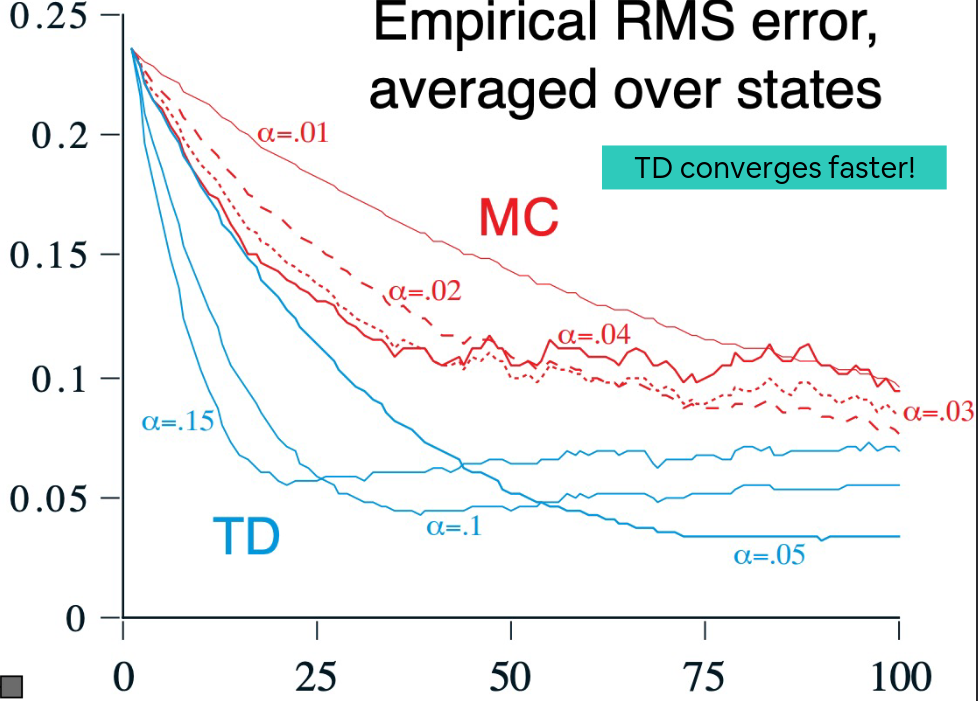
\includegraphics[width=0.85\textwidth]{figures/chapter6/image copy.png}
    \caption{Comparison between TD(0) and Monte Carlo (MC)
    in terms of estimation error. The Root Mean Square (RMS)
    error is averaged over the 5 states and then over 100
    independent runs. TD(0) generally converges faster
    than MC for the learning rates shown.}
    \label{fig:td_vs_mc}
\end{figure}

The lower $\alpha$, the lower the final error. On the other hand, higher $\alpha$ allows faster learning.

\section{Bias/Variance Trade-off}
The return $G_t$ is an unbiased estimate of $v_\pi(S_t)$. The true target $R_{t+1}+\gamma v_\pi(S_{t+1})$ is also an unbiased estimate of $v_\pi(S_t)$. However, the TD target $R_{t+1}+\gamma V(S_{t+1})$ is a biased estimate of $v_\pi(S_t)$, since it uses the current estimate $V(S_{t+1})$ instead of the true value $v_\pi(S_{t+1})$. The positve aspect of TD target is that it has much lower variane than the return $G_t$ since it depends on one random action, transition, reward:
\begin{itemize}
    \item MC has high variance and low bias
    \begin{enumerate}
        \item Good convergence properties;
        \item Not very sensitive to initial values;
        \item Simple to use and understand;
    \end{enumerate}
    \item TD has low variance and some bias
    \begin{enumerate}
        \item Usually more efficient than MC;
        \item TD(0) converges to $v_\pi(s)$;
        \item More sensitive to initial values;
    \end{enumerate}
\end{itemize}
In general we can state that unified view of the Reinforcement Learning:

\noindent
\underline{\textbf{Bootstrap}} (update involves an estimate)

\begin{itemize}
    \item \textcolor{red}{MC does not bootstrap}
    \item \textcolor{green!70!black}{DP bootstraps}
    \item \textcolor{green!70!black}{TD bootstraps}
\end{itemize}

\medskip

\noindent
\underline{\textbf{Sampling}} (use samples to estimate expectation)

\begin{itemize}
    \item \textcolor{green!70!black}{MC samples}
    \item \textcolor{red}{DP does not sample}
    \item \textcolor{green!70!black}{TD samples}
\end{itemize}

\section{TD-Learning Control}
We apply  the GPI (generalized policy iteration) approach (iteration between prediction and improvement) for solving control. Since we are model-free we use interactions over $q_\pi$. We start by considering the on-policy case. As in MC, also in this case we can consider approaches for dealing with exploration, like $\epsilon$-greedy.
\subsection{Control: SARSA-On-policy TD learning}
We need to consider transactions from (state,action) to (state,action), the update rule is:
\[Q(S_t,A_t)\leftarrow Q(S_t,A_t)+\alpha\left[R_{t+1}+\gamma Q(S_{t+1},A_{t+1})-Q(S_t,A_t)\right]\]
Pay attention that $A_{t+1}$ is the action taken according to the current policy $\pi$. 

\begin{figure}[htbp]
\centering
\begin{tikzpicture}[
    scale=0.5,
    transform shape,
    line width=1.5pt,
    every node/.style={font=\Large}
]

% Connections
\draw (0,0) -- (0,-5);

% Nodes
\filldraw[black] (0,0) circle (0.35);
\draw[fill=white] (0,-2.5) circle (0.65);
\filldraw[black] (0,-5) circle (0.35);

% Labels
\node[anchor=west] at (0.8,0) {$S,A$};
\node[anchor=west] at (1.1,-1.25) {$R$};
\node[anchor=west] at (1.0,-2.5) {$S'$};
\node[anchor=west] at (0.8,-5) {$A'$};

\end{tikzpicture}
\end{figure}

In the algorithm there will be the following elements:
\begin{itemize}
    \item GPI: policy evaluation + policy improvement;
    \item for loops for both episodes and steps of the episode;
    \item we will also need to consider the incremental updates (so we also need to set up an $\alpha$ parameter);
    \item for exploaration we will use $\epsilon$-greedy approach.
\end{itemize}

\begin{algobox}{Sarsa (on-policy TD control), for estimating $Q \approx q_*$}
\raggedright
Algorithm parameters: step size $\alpha \in (0,1]$, small $\varepsilon > 0$

\medskip
Initialize $Q(s,a)$, for all $s \in \mathcal{S}^+,\, a \in \mathcal{A}(s)$, arbitrarily except that $Q(\text{terminal},\cdot) = 0$

\medskip
Loop for each episode:\\
\hspace*{1.5em}Initialize $S$\\
\hspace*{1.5em}Choose $A$ from $S$ using policy derived from $Q$ (e.g., $\varepsilon$-greedy)\\
\hspace*{1.5em}Loop for each step of episode:\\
\hspace*{3em}Take action $A$, observe $R, S'$\\
\hspace*{3em}Choose $A'$ from $S'$ using policy derived from $Q$ (e.g., $\varepsilon$-greedy)\\
\hspace*{3em}$Q(S,A) \leftarrow Q(S,A) + \alpha \bigl[R + \gamma Q(S',A') - Q(S,A)\bigr]$\\
\hspace*{3em}$S \leftarrow S';\quad A \leftarrow A'$\\
\hspace*{1.5em}until $S$ is terminal
\end{algobox}



% bibliography.bib is empty: uncomment once it has entries
% \nocite{*}
% \bibliographystyle{plain}
% \bibliography{bibliography}
\end{document}